%
%===================================================================================================
%
\documentclass[aspectratio=169, 11pt]{beamer}

%
%===================================================================================================
%
% Theme & Colors 

\usetheme{Madrid}
\usecolortheme{whale}

\definecolor{darkblue}{RGB}{0,51,102}
\definecolor{lightgray}{RGB}{240,240,240}
\definecolor{accent}{RGB}{180,40,40}
\definecolor{darkgreen}{RGB}{0,100,60}

\setbeamercolor{frametitle}{bg=darkblue, fg=white}
\setbeamercolor{title}{bg=darkblue, fg=white}
\setbeamercolor{block title}{bg=darkblue, fg=white}
\setbeamercolor{block body}{bg=lightgray}
\setbeamercolor{block title alerted}{bg=accent, fg=white}
\setbeamercolor{block body alerted}{bg=red!5}
\setbeamercolor{block title example}{bg=darkgreen, fg=white}
\setbeamercolor{block body example}{bg=green!5}
\setbeamertemplate{navigation symbols}{}
\setbeamertemplate{footline}[frame number]

%
%===================================================================================================
%
% Packages 

\usepackage[utf8]{inputenc}
\usepackage[T1]{fontenc}
\usepackage{graphicx}
\usepackage{booktabs}
\usepackage{listings}
\usepackage{xcolor}
\usepackage{tikz}
\usetikzlibrary{arrows.meta, positioning, shapes.geometric, calc, fit, decorations.pathreplacing}
\usepackage{amsmath, amssymb}

%
%===================================================================================================
%
% Listings style 

\lstset{
  language=Python,
  basicstyle=\ttfamily\scriptsize,
  keywordstyle=\color{blue}\bfseries,
  stringstyle=\color{red!70!black},
  commentstyle=\color{green!50!black}\itshape,
  backgroundcolor=\color{lightgray},
  frame=single,
  framerule=0.4pt,
  rulecolor=\color{gray},
  breaklines=true,
  showstringspaces=false,
  columns=fullflexible,
  xleftmargin=4pt,
  xrightmargin=4pt,
  aboveskip=6pt,
  belowskip=4pt,
}

%
%===================================================================================================
%
% Title page information

\author{Giovanni Della Lunga\\{\footnotesize giovanni.dellalunga@unibo.it}}
\title{Chapter 4\\Learning and Evaluating Cross-Sectional Return Predictors}
\subtitle{Asset Pricing \& Machine Learning in Finance} % (optional)
\setbeamercovered{transparent} 
\institute{Advanced Topics in Artificial Intelligence} 
\date{Bologna - March, 2026} 
%
%===================================================================================================
%
\begin{document}
%
%===================================================================================================
%
\setbeamertemplate{subsection page}
{
  \begingroup
    %\begin{beamercolorbox}[sep=12pt,center]{section title}
      %\usebeamerfont{section title}
	  \centering 	     
      Section~\insertsectionnumber.\insertsubsectionnumber\par 
      \vspace{1cm}
    %\end{beamercolorbox}
    %\vspace*{-2pt}
    \begin{beamercolorbox}[sep=8pt,center,rounded=true]{title}
      \usebeamerfont{section title}
      \insertsubsection\par
    \end{beamercolorbox}
  \endgroup
}
%
%===================================================================================================
%
\AtBeginSection[]
{
  %\begin{frame}<beamer>
  %\footnotesize	
  %\frametitle{Outline}
  %\begin{multicols}{2}
  %\tableofcontents[currentsection]
  %\end{multicols}	  
  %\normalsize
  %\end{frame}
  \begin{frame}
  \vfill
  \centering
  \begin{beamercolorbox}[sep=8pt,center,shadow=true,rounded=true]{title}  	\usebeamerfont{title}\insertsectionhead\par%
  \end{beamercolorbox}
  \vfill
  \end{frame}
}
\AtBeginSubsection{\frame{\subsectionpage}}
%
%===================================================================================================
%
\begin{frame}
\titlepage
\end{frame}
%
%===================================================================================================
%
\begin{frame}{Contents}
%\begin{multicols}{2}
\tableofcontents[
    sectionstyle=show,
    subsectionstyle=show
]
%\end{multicols}
\end{frame}
%__________________________________________________________________________
%
\section{Model Architecture, Training \& Evaluation}
%__________________________________________________________________________
%
\begin{frame}{Where We Are in the Project}

\begin{columns}[T]
\column{0.52\textwidth}
\begin{block}{Part~1 (Previous Chapter)}
\begin{itemize}
  \item Downloaded prices \& metadata
  \item Constructed weekly returns
  \item Engineered 15 firm-level characteristics
  \item Stored everything in HDF5
\end{itemize}
\end{block}

\begin{alertblock}{Part~2 (This Chapter)}
\begin{itemize}
  \item Load \& preprocess the dataset
  \item Build the conditional autoencoder in Keras
  \item Walk-forward cross-validation
  \item Hyperparameter search \& evaluation
  \item Generate out-of-sample predictions
\end{itemize}
\end{alertblock}

\column{0.44\textwidth}
\centering
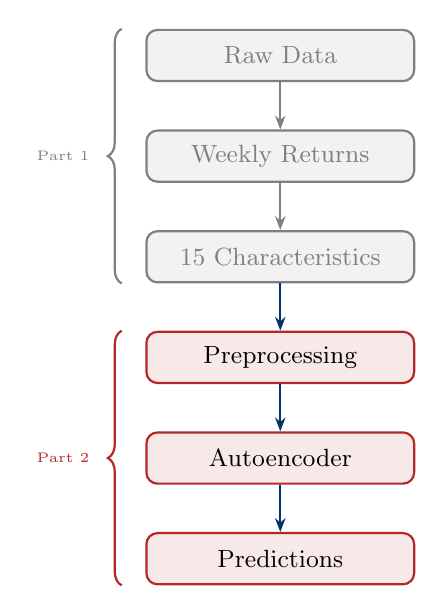
\begin{tikzpicture}[
  node distance=0.6cm,
  box/.style={draw=darkblue, thick, rounded corners, fill=darkblue!10,
              minimum width=3.4cm, minimum height=0.65cm, align=center, font=\small},
  done/.style={box, draw=gray, fill=gray!10, text=gray},
  curr/.style={box, draw=accent, fill=accent!10},
  arr/.style={-{Stealth[length=5pt]}, thick, darkblue}
]
\node[done] (d1) {Raw Data};
\node[done, below=of d1] (d2) {Weekly Returns};
\node[done, below=of d2] (d3) {15 Characteristics};
\node[curr, below=of d3] (d4) {Preprocessing};
\node[curr, below=of d4] (d5) {Autoencoder};
\node[curr, below=of d5] (d6) {Predictions};

\draw[arr, gray] (d1) -- (d2);
\draw[arr, gray] (d2) -- (d3);
\draw[arr] (d3) -- (d4);
\draw[arr] (d4) -- (d5);
\draw[arr] (d5) -- (d6);

\draw[decorate, decoration={brace, amplitude=5pt, mirror}, thick, gray]
  ([xshift=-0.3cm]d1.north west) -- ([xshift=-0.3cm]d3.south west)
  node[midway, left=8pt, font=\tiny, gray] {Part 1};
\draw[decorate, decoration={brace, amplitude=5pt, mirror}, thick, accent]
  ([xshift=-0.3cm]d4.north west) -- ([xshift=-0.3cm]d6.south west)
  node[midway, left=8pt, font=\tiny, accent] {Part 2};
\end{tikzpicture}
\end{columns}

\end{frame}
%
%..................................................................
%
\begin{frame}{1. Setup and Imports (Cells 0--8)}

The notebook begins by importing all the necessary libraries. The main ones are:

\vspace{0.3cm}

\begin{itemize}
    \item \textbf{TensorFlow/Keras}: for building and training the neural network
    \item \textbf{Pandas and NumPy}: for data manipulation
    \item \textbf{Scikit-learn} (\texttt{quantile\_transform}): for rank normalization
    \item \textbf{SciPy} (\texttt{spearmanr}): for computing the Information Coefficient
    \item \textbf{Matplotlib and Seaborn}: for plotting
\end{itemize}

\end{frame}
%
%..................................................................
%
\begin{frame}{Feature Selection and Setup}

Then, the list of 15 features to be used as input to the beta network is defined:

\vspace{0.3cm}

\begin{block}{Python}
\small
\texttt{
characteristics = ['beta', 'betasq', 'chmom', 'dolvol', 'idiovol', 'ill', 'indmom', \\
\hspace{1.2cm} 'maxret', 'mom12m', 'mom1m', 'mom36m', 'mvel', 'retvol', 'turn']
}
\end{block}

\vspace{0.3cm}

These are the same variables constructed in the previous notebook (Part 1, data preparation): 6 price trend factors, 5 liquidity factors, and 4 risk factors — all computed using rolling windows on historical data.

\vspace{0.3cm}

Finally, the path where all results will be saved is set, and the random seed is fixed at 42 for reproducibility.

\end{frame}
%
%..................................................................
%
\begin{frame}{2. Data Loading (Cells 9--14)}

The notebook loads weekly returns from the HDF5 file produced during the data preparation phase:

\vspace{0.3cm}

\begin{block}{Python}
\small
\texttt{
data = (pd.read\_hdf(results\_path / 'autoencoder\_reloaded.h5', 'returns') \\
\hspace{0.8cm} .stack(dropna=False) \\
\hspace{0.8cm} .to\_frame('returns') \\
\hspace{0.8cm} .loc[idx['1993':, :], :])
}
\end{block}

\vspace{0.3cm}

The result is a DataFrame with a MultiIndex (\texttt{date, ticker}) and one column \texttt{returns}.  
The structure is in "long" format: each row corresponds to one asset in a specific week.

\vspace{0.3cm}

The choice of starting from 1993 is due to the fact that many features require 3-year rolling windows, so data before 1993 do not have sufficient history for computation.

\end{frame}
%
%..................................................................
%
\begin{frame}{3. Exploratory Analysis of a Single Asset (Cells 15--18)}

The notebook isolates Apple (AAPL) returns and visualizes them in two ways: a time series plot of weekly returns and a histogram of their distribution.

\vspace{0.3cm}

This is a simple sanity check — it allows us to visually verify that the data are reasonable, without anomalous spikes or obvious gaps.

\end{frame}
%
%..................................................................
%
\begin{frame}{4. Feature Merging (Cells 19--25)}

The 15 features are loaded from the HDF5 file and added to the main DataFrame. In the file, each feature is stored with a key starting with \texttt{factor/} (e.g., \texttt{factor/beta}, \texttt{factor/mom12m}):

\vspace{0.3cm}

\begin{block}{Python}
\small
\texttt{
with pd.HDFStore(results\_path / 'autoencoder\_reloaded.h5') as store: \\
\hspace{0.8cm} keys = [k[1:] for k in store.keys() if k[1:].startswith('factor/')] \\
\hspace{0.8cm} for key in keys: \\
\hspace{1.6cm} data[key.split('/')[-1]] = store[key].squeeze()
}
\end{block}

\vspace{0.3cm}

After this step, the DataFrame \texttt{data} has one row per (week, asset) pair and 16 columns: \texttt{returns} plus the 15 features.

\vspace{0.3cm}

The notebook then updates the \texttt{characteristics} list by directly reading the DataFrame columns (excluding \texttt{returns}).

\end{frame}
%
%..................................................................
%
\begin{frame}{5. Target Creation: Forward Returns (Cell 26)}

This is a fundamental line:

\vspace{0.3cm}

\begin{block}{Python}
\small
\texttt{
data['returns\_fwd'] = data.returns.unstack('ticker').shift(-1).stack()
}
\end{block}

\vspace{0.3cm}

What it does in detail: it takes returns, pivots them into wide format (date $\times$ ticker), shifts everything up by one row (so that next week's return is aligned with the current week), and then converts back to long format.

\vspace{0.3cm}

The result is a new column \texttt{returns\_fwd}, where for each row corresponding to week $t$ and asset $i$, we find the return at time $t+1$.

\vspace{0.3cm}

This is the model's target: the network learns to use today's features to predict tomorrow's return. Without this shift, the model would attempt to "predict the present," which has no practical value.

\end{frame}
%
%..................................................................
%
\begin{frame}{6. Data Coverage Analysis (Cells 29--32)}

The notebook computes and visualizes:

\vspace{0.3cm}

\begin{itemize}
    \item How many assets are available in each week (distribution of the number of observations per date)
    \item How many observations each feature has over time (to verify that there are no features with too many missing values)
\end{itemize}

\vspace{0.3cm}

This serves as a quality check: if a feature had very few observations in certain weeks, it could be unreliable and should be treated differently.

\end{frame}
%
%..................................................................
%
\begin{frame}{7. Rank Normalization (Cell 34)}

This is one of the most important steps:

\begin{block}{Python}
\scriptsize
\texttt{
data.loc[:, characteristics] = ( \\
\hspace{0.5cm} data.loc[:, characteristics] \\
\hspace{1.0cm} .groupby(level='date') \\
\hspace{1.0cm} .apply(lambda x: pd.DataFrame( \\
\hspace{1.5cm} quantile\_transform(x, copy=True, n\_quantiles=x.shape[0]), \\
\hspace{1.5cm} columns=characteristics, \\
\hspace{1.5cm} index=x.index.get\_level\_values('ticker') \\
\hspace{1.0cm} )) \\
\hspace{1.0cm} .mul(2).sub(1) \\
)
}
\end{block}
\footnotesize
For each week separately (\texttt{groupby(level='date')}), each feature is transformed into its empirical quantiles via \texttt{quantile\_transform}. This produces values in $[0,1]$, where 0 corresponds to the lowest value and 1 to the highest. Then, \texttt{.mul(2).sub(1)} rescales the interval from $[0,1]$ to $(-1,1)$.

The result is that all 15 features become comparable, bounded in the same range, free of outliers, and with a uniform cross-sectional distribution each week. This is essential for stable neural network training.

\end{frame}
%
%..................................................................
%
\begin{frame}{9. Model Architecture (Cells 42--61)}

The notebook builds a conditional autoencoder in Keras. Let us examine each component.


\vspace{0.3cm}

\textbf{Inputs (Cell 49):}

\vspace{0.2cm}

\begin{block}{Python}
%\small
\texttt{input\_beta = Input((n\_tickers, n\_characteristics), name='input\_beta') \\
input\_factor = Input((n\_tickers,), name='input\_factor')
}
\end{block}

\vspace{0.3cm}

Two separate input layers: \texttt{input\_beta} receives a matrix (all assets $\times$ 15 features) for each week. \texttt{input\_factor} receives a vector of returns (one value per asset) for each week.

\end{frame}
%
%..................................................................
%
\begin{frame}{Beta Network (Cell 51)}

\begin{block}{Python}
\small
\texttt{hidden\_layer = Dense(units=8, activation='relu', name='hidden\_layer')(input\_beta) \\
batch\_norm = BatchNormalization(name='batch\_norm')(hidden\_layer) \\
output\_beta = Dense(units=n\_factors, name='output\_beta')(batch\_norm)
}
\end{block}

\vspace{0.3cm}

Three steps in sequence. The Dense layer with 8 neurons and ReLU transforms the 15 features into 8 non-linear features, applying the same weights to each asset (weight sharing).

\vspace{0.3cm}

Batch Normalization standardizes these activations to stabilize training.

\vspace{0.3cm}

The final Dense layer (linear, no activation) produces $K$ factor loadings for each asset.

\vspace{0.3cm}

Output shape: (batch, n\_tickers, $K$).

\end{frame}
%
%..................................................................
%
\begin{frame}{Factor Network (Cell 53)}

\begin{block}{Python}
\small
\texttt{
output\_factor = Dense(units=n\_factors, name='output\_factor')(input\_factor)
}
\end{block}

\vspace{0.3cm}

A single linear layer that takes returns of all assets and combines them into $K$ latent factors.

\vspace{0.3cm}

Output shape: (batch, $K$).

\end{frame}
%
%..................................................................
%
\begin{frame}{Dot Product (Cell 55)}

\begin{block}{Python}
\small
\texttt{
output = Dot(axes=(2,1), name='output\_layer')([output\_beta, output\_factor])
}
\end{block}

\vspace{0.3cm}

For each asset, this computes the dot product between its beta vector ($K$ values) and the factor vector ($K$ values), producing the predicted return.

\vspace{0.3cm}

The argument \texttt{axes=(2,1)} instructs Keras to contract dimension 2 of \texttt{output\_beta} (the $K$ factors) with dimension 1 of \texttt{output\_factor} (also $K$).

\vspace{0.3cm}

Output shape: (batch, n\_tickers) — one predicted return for each asset in each week.

\end{frame}
%
%..................................................................
%
\begin{frame}{Model Compilation (Cell 57)}

\begin{block}{Python}
\small
\texttt{
model = Model(inputs=[input\_beta, input\_factor], outputs=output) \\
model.compile(loss='mse', optimizer='adam')
}
\end{block}

\vspace{0.3cm}

The loss function is MSE (Mean Squared Error):
\[
\frac{1}{N} \sum_i (r_{i,t} - \hat{r}_{i,t})^2
\]

\vspace{0.3cm}

The optimizer is Adam, a variant of SGD with an adaptive learning rate.

\vspace{0.3cm}

\textbf{Helper Function (Cell 59):} \texttt{make\_model(hidden\_units, n\_factors)} encapsulates the entire architecture into a parametric function, allowing easy creation of models with different hyperparameter combinations.

\end{frame}
%
%..................................................................
%
\begin{frame}{10. Cross-Validation Setup (Cells 62--68)}

\textbf{Time Series CV (Cell 67):}

\vspace{0.2cm}

\begin{block}{Python}
\small
\texttt{
cv = MultipleTimeSeriesCV(n\_splits=5, \\
\hspace{0.8cm} train\_period\_length=20*YEAR, \\
\hspace{0.8cm} test\_period\_length=1*YEAR, \\
\hspace{0.8cm} lookahead=2)
}
\end{block}

\vspace{0.3cm}

Creates a 5-fold walk-forward setup: 20 years of training, a 2-week gap, and 1 year of testing. The windows move forward in time at each fold.

\vspace{0.3cm}

\textbf{Data Splitting Function (Cell 68):} \texttt{get\_train\_valid\_data} takes training and validation indices and returns six objects: for each of the two sets (train and validation), it produces features as 3D tensors (weeks $\times$ assets $\times$ 15), returns as 2D matrices (weeks $\times$ assets), and forward returns as targets.

\end{frame}
%
%..................................................................
%
\begin{frame}{Time-Series Cross-Validation Design}
\vspace{0.5cm}
\centering
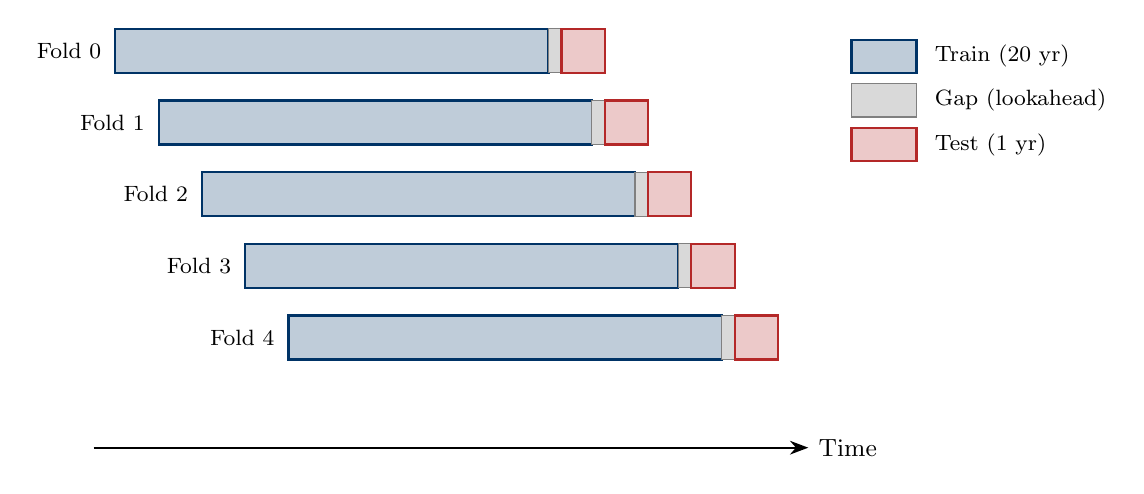
\begin{tikzpicture}[
  xscale=0.55, yscale=0.7,
  train/.style={fill=darkblue!25, draw=darkblue, thick},
  gap/.style={fill=gray!30, draw=gray},
  test/.style={fill=accent!25, draw=accent, thick},
  lbl/.style={font=\footnotesize}
]

\foreach \f/\ts/\te/\vs/\ve in {
  0/0/10/10.3/11.3,
  1/1/11/11.3/12.3,
  2/2/12/12.3/13.3,
  3/3/13/13.3/14.3,
  4/4/14/14.3/15.3
}{
  \draw[train] (\ts, -\f*1.3) rectangle (\te, -\f*1.3+0.8);
  \draw[gap]   (\te, -\f*1.3) rectangle (\vs, -\f*1.3+0.8);
  \draw[test]  (\vs, -\f*1.3) rectangle (\ve, -\f*1.3+0.8);
  \node[lbl, left] at (\ts-0.1, -\f*1.3+0.4) {Fold \f};
}

% Legend
\draw[train] (17, 0) rectangle (18.5, 0.6);
\node[font=\footnotesize, right] at (18.7, 0.3) {Train (20 yr)};
\draw[gap]   (17, -0.8) rectangle (18.5, -0.2);
\node[font=\footnotesize, right] at (18.7, -0.5) {Gap (lookahead)};
\draw[test]  (17, -1.6) rectangle (18.5, -1.0);
\node[font=\footnotesize, right] at (18.7, -1.3) {Test (1 yr)};

% Time arrow
\draw[-{Stealth}, thick] (-0.5, -6.8) -- (16, -6.8) node[right, font=\small] {Time};

\end{tikzpicture}
\end{frame}
%
%..................................................................
%
\begin{frame}{Time-Series Cross-Validation Design}

\begin{block}{\texttt{MultipleTimeSeriesCV} Parameters}
\centering\small
\begin{tabular}{lcl}
\toprule
\textbf{Parameter} & \textbf{Value} & \textbf{Meaning} \\
\midrule
\texttt{n\_splits} & 5 & Number of walk-forward folds \\
\texttt{train\_period\_length} & $20 \times 52 = 1040$ weeks & Training window \\
\texttt{test\_period\_length} & $1 \times 52 = 52$ weeks & Validation window \\
\texttt{lookahead} & 2 & Gap to prevent information leakage \\
\bottomrule
\end{tabular}
\end{block}

\end{frame}
%
%..................................................................
%
\begin{frame}{11. Grid Search and Training (Cells 69--80)}

\textbf{Hyperparameter Grid (Cell 70):}

\vspace{0.2cm}

\begin{block}{Python}
\small
\texttt{
factor\_opts = [2, 3, 4, 5, 6] \\
unit\_opts = [8, 16, 32]
}
\end{block}

\vspace{0.3cm}

In total, $5 \times 3 = 15$ combinations are tested.

\end{frame}
%
%..................................................................
%
\begin{frame}{Main Training Loop (Cell 79)}

For each combination (\texttt{units}, \texttt{n\_factors}):

\vspace{0.3cm}

\begin{enumerate}
    \item Create a new model
    \item For each CV fold:
    \begin{itemize}
    \normalsize
        \item Split the data into training and validation sets
        \item Train the model incrementally for 250 epochs
        \item After each epoch, generate predictions on the validation set
        \item Compute two metrics:
        \begin{itemize}
        \normalsize
            \item \textbf{Pooled IC} (\texttt{r0}): Spearman correlation between all predictions and all realized returns, pooled together
            \item \textbf{IC by date} (\texttt{r1\_by\_date}): Spearman correlation computed separately for each week, then summarized using mean, median, and standard deviation
        \end{itemize}
        \item Save the results
    \end{itemize}
\end{enumerate}

\end{frame}
%
%..................................................................
%
\begin{frame}[fragile]{Incremental Training in Cross-Validation (Cell 79)}

The relevant code is:

\begin{block}{Python}
\scriptsize
\begin{verbatim}
model = make_model(hidden_units=units, n_factors=n_factors)
for fold, (train_idx, val_idx) in enumerate(cv.split(data)):
    X1_train, X2_train, y_train, X1_val, X2_val, y_val = get_train_valid_data(...)
    for epoch in range(250):
        model.fit([X1_train, X2_train], y_train,
                  batch_size=batch_size,
                  epochs=epoch + 1,
                  initial_epoch=epoch,
                  verbose=0)
        # compute IC on validation set
        y_pred = model.predict([X1_val, X2_val])
        # ... save metrics for this epoch
\end{verbatim}
\end{block}

The key lies in the pair of parameters \texttt{epochs=epoch+1} and \texttt{initial\_epoch=epoch}. Let us examine what happens during the first iterations of the loop.

\end{frame}
%
%..................................................................
%
\begin{frame}{How Incremental Training Works}

When \textbf{epoch = 0}: Keras trains from \textbf{initial\_epoch=0} to \textbf{epochs=1}, that is, it performs a single pass over the entire training set. The weights start from their random initialization and are updated once. Then the code exits \texttt{model.fit}, computes the IC on the validation set, and saves it.

\vspace{0.3cm}

When \textbf{epoch = 1}: Keras trains from \textbf{initial\_epoch=1} to \textbf{epochs=2}. The weights are \textbf{not reset} — they start exactly from where they stopped at the end of the previous iteration. Another pass is performed on the training data, and the weights are updated further. Then the IC is computed again.

\vspace{0.3cm}

When \textbf{epoch = 2}: training resumes from the current state, performs one more pass, and continues in the same way up to epoch 249.

\end{frame}
%
%..................................................................
%
\begin{frame}{Why Not Simply Use \texttt{model.fit(epochs=250)}?}

Because you would lose crucial information. Imagine that the IC on the validation set increases up to epoch 70 and then starts to decline. If you only evaluate at epoch 250, you would observe a mediocre IC and miss the fact that the model performed much better 180 epochs earlier. Incremental training provides a full picture of the model’s evolution over time.

\vspace{0.3cm}

To better understand, think of training like baking a cake in the oven. Incremental training is like opening the oven every minute, checking the cake, and noting its condition. In the end, you can say: ``the cake was perfect at minute 35''. If you only checked at the end (minute 120), you might find a burnt cake without knowing when it was at its best.

\end{frame}
%
%..................................................................
%
\begin{frame}{Incremental Training and Information Coefficient}

Training is incremental: \texttt{model.fit(epochs=epoch+1, initial\_epoch=epoch)} advances training one epoch at a time without resetting the weights, allowing metrics to be tracked at each step.

\vspace{0.3cm}

The Information Coefficient (IC) measures the model's ability to correctly rank assets: if the model assigns higher expected returns to assets that actually perform better, the IC is positive.

\vspace{0.3cm}

In quantitative practice, an average daily IC of 0.03--0.05 is already considered good.

\end{frame}
%
%..................................................................
%
\begin{frame}{12. Results Evaluation (Cells 81--96)}

The notebook loads all scores saved during cross-validation and analyzes them.

\vspace{0.3cm}

\textbf{Aggregation Across Folds (Cell 87):}

\vspace{0.2cm}

\begin{block}{Python}
\small
\texttt{
avg = (scores.groupby(['n\_factors', 'units', 'epoch'])[columns\_to\_average] \\
\hspace{0.8cm} .mean().reset\_index())
}
\end{block}

\vspace{0.3cm}

For each combination (\texttt{n\_factors}, \texttt{units}, \texttt{epoch}), it computes the average IC across the 5 folds. This reduces fold-to-fold noise.

\vspace{0.3cm}

\textbf{Top-5 Epochs per Configuration (Cell 91):} For each hyperparameter pair, it selects the 5 epochs with the highest median daily IC.

\end{frame}
%
%..................................................................
%
\begin{frame}{Visualization and Key Findings}

\textbf{Visualization (Cell 95):} A 5$\times$2 plot shows the learning curves (IC vs.\ epoch) for all combinations. The top row displays pooled IC, while the bottom row shows median daily IC (more robust). Colored lines distinguish 8, 16, and 32 hidden units.

\vspace{0.3cm}

\textbf{Key Findings (Cell 96):}

\vspace{0.2cm}

\begin{itemize}
    \item 32 hidden units tend to produce unstable or worse results — excessive capacity leads to overfitting
    \item IC typically peaks between epochs 40 and 100, then declines
    \item The configuration with \textbf{4 factors and 16 hidden units} is the most consistently positive in terms of median daily IC
    \item 5 factors with 8 units can yield higher pooled IC, but require more aggressive early stopping
\end{itemize}

\end{frame}
%
%..................................................................
%
\begin{frame}{13. Final Predictions Generation (Cells 97--103)}

With the selected hyperparameters (4 factors, 16 units), the notebook generates the final predictions:

\vspace{0.3cm}

\begin{block}{Python}
\small
\texttt{
for epoch in range(50, 100): \\
\hspace{0.8cm} for fold, (train\_idx, val\_idx) in enumerate(cv.split(data)): \\
\hspace{1.6cm} model = make\_model(...) \\
\hspace{1.6cm} model.fit(..., epochs=epoch) \\
\hspace{1.6cm} predictions = model.predict(...)
}
\end{block}

\vspace{0.3cm}

For each epoch from 50 to 99, and for each fold, a new model is trained from scratch for exactly that number of epochs and then used to predict on the validation set. In total, $50 \times 5 = 250$ prediction sets are generated, concatenated, and averaged.

\vspace{0.3cm}

This ensemble averaging strategy leverages diversity across models (different initializations and training lengths) to produce more stable and robust predictions.

\vspace{0.3cm}

The final result is saved in \texttt{predictions\_reloaded.h5}.

\end{frame}
%
%..................................................................
%
\begin{frame}[fragile]{Difference with Cross-Validation (Cell 100)}

In the final stage, the strategy is completely different:

\vspace{0.3cm}

\begin{block}{Python}
\scriptsize
\begin{verbatim}
for epoch in range(50, 100):
    for fold, (train_idx, val_idx) in enumerate(cv.split(data)):
        model = make_model(...)   # NEW model at each iteration
        model.fit(..., epochs=epoch)  # train from scratch for 'epoch' epochs
        predictions = model.predict(...)
\end{verbatim}
\end{block}

\vspace{0.3cm}

Here, \texttt{make\_model(...)} is inside both loops. Each time, a model with new random weights is created, trained from scratch for a fixed number of epochs, and then used for prediction.

\vspace{0.3cm}

There is nothing incremental — this results in $50 \times 5 = 250$ completely independent training runs.

\end{frame}
%
%..................................................................
%
\begin{frame}[fragile]{What Happens in Practice}

The loop creates \textbf{50 different models} (one for each epoch from 50 to 99), and for each of them repeats the procedure across all 5 folds. In detail:

\vspace{0.3cm}

When \texttt{epoch = 50}: a new model is created with randomly initialized weights, trained from scratch for exactly 50 epochs, and then used to generate predictions on the validation set.

\vspace{0.3cm}

When \texttt{epoch = 51}: another new model is created (with different random weights), trained from scratch for 51 epochs, and predictions are generated.

\vspace{0.3cm}

When \texttt{epoch = 52}: same procedure, trained for 52 epochs. This continues up to \texttt{epoch = 99}.

\vspace{0.3cm}

At the end (Cell 101), all predictions are concatenated and averaged:

\vspace{0.2cm}

\begin{block}{Python}
\small
\begin{verbatim}
predictions_combined = pd.concat(predictions, axis=1).sort_index()
\end{verbatim}
\end{block}

\end{frame}
%
%..................................................................
%
\begin{frame}{Why Do This? The Ensemble Idea}

From the cross-validation phase, it emerged that the model with 4 factors and 16 hidden units performs well, and that the best results are obtained by stopping training roughly between epochs 50 and 100. However, there is no single magic number — epoch 73 may be slightly better than epoch 68 for one fold, and worse for another.

\vspace{0.3cm}

Instead of betting on a single stopping epoch, the notebook adopts an \textbf{ensemble averaging} strategy: it generates predictions from 50 models (each trained for a slightly different number of epochs) and then averages them.

\vspace{0.3cm}

This has two advantages. First, it reduces variance: a single model may produce noisy predictions, but averaging 50 models stabilizes them. Second, it makes the result robust to the exact choice of early stopping: it does not matter whether the perfect epoch was 67 or 82, because both contribute to the final average.

\end{frame}
%
%..................................................................
%
\begin{frame}{An Important Point}

Note that at each iteration the model is recreated from scratch (\texttt{make\_model(...)} inside the loop). This means that the 50 models differ not only in the number of training epochs, but also in the random initialization of their weights.

\vspace{0.3cm}

This adds an additional source of diversity to the ensemble, making it even more robust.

\end{frame}
%
%..................................................................
%
\begin{frame}{What the Final Predictions Represent}

The DataFrame \texttt{\textcolor{red}{predictions\_combined}} saved in cell 103 has a precise structure:
the index is a MultiIndex \texttt{(date, ticker)}, and the columns are 250 prediction vectors
\mbox{(50 epochs $\times$ 5 folds).} Each cell contains the predicted weekly return
$\hat{r}_{i,t+1}$ for stock $i$ at week $t$.

\vspace{0.4cm}

To obtain the model's final prediction for each pair \mbox{$($date, stock$)$,} we take the average
across the columns:

\vspace{0.5cm}

\[
\hat{r}^{\mathrm{ensemble}}_{i,t+1}
=
\frac{1}{250}\sum_{m=1}^{250}\hat{r}^{(m)}_{i,t+1}
\]

\vspace{0.5cm}

This average has two effects. First, it reduces the idiosyncratic noise of each individual
model. Second, it makes the result robust to the choice of stopping epoch --- it does not
matter whether the optimal epoch was 63 or 78, because both contribute.

\end{frame}
%
%..................................................................
%
\begin{frame}{What the Predictions Are Not}

A fundamental point to understand is that these predictions \textbf{are not reliable point estimates}
of the future return of each individual stock. It would be unrealistic to expect the model
to say ``Apple will return +2.3\% next week.'' The stock market contains far too much noise
for that.

\vspace{0.4cm}

What the model does well is \textbf{rank stocks}: among 2{,}500 equities, those to which it assigns
higher predictions do tend, on average, to perform better than those to which it assigns lower
predictions. It is a ranking signal, not a level estimate. This is exactly what the IC measures.

\end{frame}
%
%..................................................................
%
\begin{frame}{How They Are Used in Practice}

The autoencoder's predictions are used as inputs for portfolio construction.
The typical implementation involves several steps.

\vspace{0.25cm}

\textbf{Long-short portfolio:} each week, stocks are sorted by predicted return. One buys
those in the top quintile (top 20\%) and short-sells those in the bottom quintile
(bottom 20\%). The return of this portfolio is the ``factor-mimicking portfolio'' ---
if the IC is positive, this portfolio will have a positive expected return.

\vspace{0.25cm}

\textbf{Sharpe ratio:} the key measure of success is the annualized Sharpe ratio of the
long-short portfolio. There is a well-known approximate relationship between IC and
Sharpe:

\vspace{0.35cm}

\[
\mathrm{SR} \approx \mathrm{IC} \times \sqrt{\mathrm{BR}}
\]

\vspace{0.35cm}

where BR is ``breadth,'' that is, the number of independent bets (approximately the
number of stocks $\times$ the number of periods). With an IC of 0.03 and about 2{,}500
stocks rebalanced weekly, interesting Sharpe ratios can be obtained.

\end{frame}
%
%..................................................................
%

%
%..................................................................
%

%
%..................................................................
%

%
%..................................................................
%

%
%..................................................................
%


%__________________________________________________________________________
%
\section{Performance Evaluation of Alpha Factors with Alphalens}
%__________________________________________________________________________
%
\begin{frame}{Alphalens Evaluation Pipeline}

\begin{columns}[T]
\column{0.48\textwidth}
\begin{block}{Setup}
\begin{itemize}
  \item Epoch-averaged predictions $\rightarrow$ single factor score per (date, ticker)
  \item Aligned with weekly trade prices (Friday, UTC)
  \item Holding periods: 5D, 10D, 21D
  \item 5 quintiles ($Q=5$)
\end{itemize}
\end{block}

\begin{block}{Alphalens Key Function}
\texttt{get\_clean\_factor\_and\_forward\_returns}\\
merges factor scores with realised forward returns and assigns quantiles. $\sim$18.5\% observations dropped (missing fwd returns).
\end{block}

\column{0.48\textwidth}
\begin{block}{Diagnostics Produced}
\begin{enumerate}
  \item \textbf{Quantile returns}: bar charts, cumulative lines, violin plots
  \item \textbf{Alpha \& Beta}: factor regressed on market return
  \item \textbf{Information Coefficient}: distribution, time series, monthly heatmap
  \item \textbf{Turnover}: quantile composition stability, rank autocorrelation
  \item \textbf{Summary \& full tear sheets}
\end{enumerate}
\end{block}
\end{columns}

\end{frame}
%
%..................................................................
%
\begin{frame}{Quantile Returns: Monotonic Cross-Sectional Ordering}

\begin{columns}[T]
\column{0.48\textwidth}
\begin{block}{Cumulative Returns by Quantile}
\begin{itemize}
  \item \textbf{5D horizon}: clear monotonic spread; Q5 outperforms, Q1 underperforms
  \item \textbf{10D}: ordering persists, spread slightly narrows
  \item \textbf{21D}: structure still visible but weaker $\Rightarrow$ signal is primarily \textbf{short-term}
\end{itemize}
\end{block}
\vspace{-.3cm}
\begin{block}{Long--Short Spread (Q5 $-$ Q1)}
\centering\small
\begin{tabular}{lc}
\toprule
Horizon & Mean Spread (bps) \\
\midrule
5D & 31.4 \\
10D & 16.8 \\
21D & 17.8 \\
\bottomrule
\end{tabular}
\end{block}

\column{0.48\textwidth}
\begin{block}{Alpha \& Beta vs.\ Market}
\centering\small
\begin{tabular}{lccc}
\toprule
& 5D & 10D & 21D \\
\midrule
Ann.\ Alpha & 3.05\% & 0.70\% & 3.44\% \\
Beta & 0.062 & 0.054 & 0.009 \\
\bottomrule
\end{tabular}

\medskip
\raggedright
Near-zero betas confirm the factor is \textbf{orthogonal to the market}: it captures \textbf{idiosyncratic}, firm-specific predictive content.
\end{block}
\end{columns}
\end{frame}
%
%..................................................................
%
\begin{frame}{Quantile Returns: Monotonic Cross-Sectional Ordering}
\vspace{0.5cm}
\begin{exampleblock}{Economic Interpretation}
The CAE compresses 15 characteristics into a latent score that ranks stocks by expected return. The ranking is stable, monotonic, and market-independent.
\end{exampleblock}
\end{frame}
%
%..................................................................
%
\begin{frame}{Information Coefficient Analysis}

\begin{columns}[T]
\column{0.48\textwidth}
\begin{block}{IC Summary Statistics}
\centering\small
\begin{tabular}{lccc}
\toprule
& 5D & 10D & 21D \\
\midrule
IC Mean & 0.008 & 0.004 & 0.009 \\
IC Std & 0.053 & 0.047 & 0.041 \\
Risk-Adj.\ IC & 0.146 & 0.095 & 0.229 \\
$t$-stat & 2.27 & 1.47 & 3.54 \\
$p$-value & 0.024 & 0.142 & 0.000 \\
\bottomrule
\end{tabular}
\end{block}

\vspace{-0.3cm}

\begin{block}{Key Observations}
\begin{itemize}
  \item IC positive at \textbf{all horizons}
  \item Statistically significant at 5D ($p{=}0.024$) and 21D ($p{<}0.001$)
  %\item IC distributions are \textbf{near-Gaussian} (Q-Q plots confirm)
  %\item IC std \textbf{decreases} with horizon $\Rightarrow$ increased signal stability
\end{itemize}
\end{block}

\column{0.48\textwidth}
\begin{block}{Temporal Dynamics}
\begin{itemize}
  \item Rolling IC oscillates around zero with recurrent \textbf{positive phases}
  \item Sustained strength 2016--2017; brief weakness during late-2018 volatility
  \item Monthly IC heatmaps: \textbf{predominantly blue} (positive), especially at 21D
  \item No persistent structural breakdowns detected
\end{itemize}
\end{block}
\end{columns}
\end{frame}
%
%..................................................................
%
\begin{frame}{Information Coefficient Analysis}

\begin{alertblock}{Interpretation}
The CAE factor provides a \textbf{statistically significant, temporally stable} predictive signal. Magnitudes ($\text{IC} \approx 0.01$) are typical for equity factors and sufficient for economically meaningful strategies when applied with high breadth.
\end{alertblock}

\end{frame}
%
%..................................................................
%
\begin{frame}{Turnover \& Signal Persistence}

\begin{columns}[T]
\column{0.48\textwidth}
\begin{block}{Quantile Turnover}
\centering\small
\begin{tabular}{lccc}
\toprule
Quantile & 5D & 10D & 21D \\
\midrule
Q1 & 0.496 & 0.572 & 0.644 \\
Q3 & 0.655 & 0.697 & 0.734 \\
Q5 & 0.490 & 0.568 & 0.640 \\
\bottomrule
\end{tabular}

\medskip
\raggedright
Turnover in the 0.49--0.75 range. Extreme quintiles (Q1, Q5) are the \textbf{most stable}, suggesting persistent rankings at the tails.
\end{block}

\column{0.48\textwidth}
\begin{block}{Factor Rank Autocorrelation}
\centering\small
\begin{tabular}{lc}
\toprule
Horizon & Mean Autocorr. \\
\midrule
5D & 0.511 \\
10D & 0.399 \\
21D & 0.286 \\
\bottomrule
\end{tabular}

\medskip
\raggedright
Smooth decay from 0.51 to 0.29: the signal persists for \textbf{1--3 weeks} before dissipating. This is consistent with short-to-medium-term equity factors.
\end{block}
\end{columns}
\end{frame}
%
%..................................................................
%
\begin{frame}{Turnover \& Signal Persistence}

\begin{exampleblock}{Balance Between Adaptability and Persistence}
The model updates frequently enough to incorporate new information while maintaining stable rankings, avoiding excessive transaction costs. Turnover spikes coincide with market volatility, not model instability.
\end{exampleblock}

\end{frame}
%
%..................................................................
%
\begin{frame}{Summary of Findings}

\begin{block}{What the Results Suggest}
The conditional autoencoder:
\begin{enumerate}
  \item \textbf{Orders the cross-section coherently}: monotonic Q1--Q5 return spreads at all horizons
  \item \textbf{Delivers market-orthogonal alpha}: annualised $\alpha \approx 3\%$, $\beta \approx 0$ vs.\ the market
  \item \textbf{Produces statistically significant ICs}: $t$-stat $> 2$ at 5D and 21D
  \item \textbf{Remains temporally stable}: no structural breakdowns across 2015--2019
  \item \textbf{Balances adaptability and persistence}: smooth turnover, rank autocorrelation decays naturally
\end{enumerate}
\end{block}

\vspace{0.2cm}

\begin{block}{Conceptual Contribution}
The CAE bridges \textbf{economic structure} (conditional factor model, no-arbitrage) with \textbf{deep learning flexibility} (nonlinear loadings, data-driven factors). It demonstrates that interpretability and complexity are \textbf{complementary}, not opposing.
\end{block}

\end{frame}
%__________________________________________________________________________
%
%\appendix
%__________________________________________________________________________
%
\section{Appendix A\\ Keras}
%__________________________________________________________________________
%
\begin{frame}{What Is Keras? --- The 5-Step Workflow}

\begin{columns}[T]
\column{0.50\textwidth}
\small
\textbf{Keras} is the high-level API of TensorFlow for building and training neural networks. Accessible as \texttt{tensorflow.keras}.

\vspace{0.15cm}

\begin{block}{\small Key Characteristics}
\footnotesize
\begin{itemize}\setlength\itemsep{1pt}
  \item \textbf{Modular}: models = layers snapped together
  \item \textbf{Two APIs}: Sequential (simple) and Functional (complex)
  \item \textbf{Extensible}: custom layers, losses, callbacks
  \item Runs on CPU, GPU, and TPU
\end{itemize}
\end{block}

\column{0.46\textwidth}
\centering
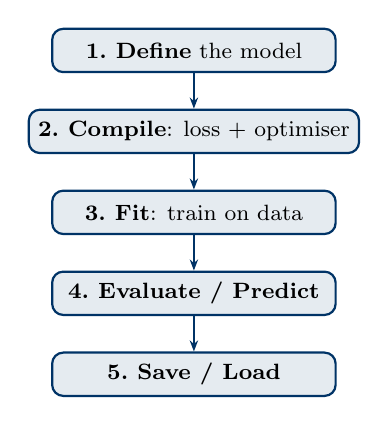
\begin{tikzpicture}[
  node distance=0.45cm,
  box/.style={draw=darkblue, thick, rounded corners, fill=darkblue!10,
              minimum width=3.6cm, minimum height=0.55cm, align=center,
              font=\footnotesize},
  arr/.style={-{Stealth[length=4pt]}, thick, darkblue}
]
\node[box] (d) {\textbf{1.\ Define} the model};
\node[box, below=of d] (c) {\textbf{2.\ Compile}: loss + optimiser};
\node[box, below=of c] (f) {\textbf{3.\ Fit}: train on data};
\node[box, below=of f] (e) {\textbf{4.\ Evaluate / Predict}};
\node[box, below=of e] (s) {\textbf{5.\ Save / Load}};
\draw[arr] (d)--(c); \draw[arr] (c)--(f);
\draw[arr] (f)--(e); \draw[arr] (e)--(s);
\end{tikzpicture}
\end{columns}

\end{frame}
%
%..................................................................
%
\begin{frame}[fragile]{Sequential vs.\ Functional API}

\begin{columns}[T]
\column{0.48\textwidth}
\begin{block}{\small Sequential --- Single Chain of Layers}
\begin{lstlisting}
from tensorflow.keras.models import Sequential
from tensorflow.keras.layers import Dense, Dropout

model = Sequential([
  Dense(64, activation='relu',
        input_shape=(15,)),
  Dropout(0.2),
  Dense(32, activation='relu'),
  Dense(1)          # regression output
])
\end{lstlisting}
\footnotesize One input, one output, no branching.
\end{block}

\column{0.48\textwidth}
\begin{block}{\small Functional --- Multi-Input / Branching}
\begin{lstlisting}
from tensorflow.keras.layers import (
    Input, Dense, BatchNormalization, Dot)
from tensorflow.keras.models import Model

inp_chars = Input((N, P), name='chars')
inp_ret   = Input((N,),   name='returns')
# Branch 1
x = Dense(8, activation='relu')(inp_chars)
x = BatchNormalization()(x)
betas = Dense(K)(x)
# Branch 2
factors = Dense(K)(inp_ret)
# Merge
out = Dot(axes=(2,1))([betas, factors])

model = Model([inp_chars, inp_ret], out)
\end{lstlisting}
\end{block}
\end{columns}

%\vspace{0.15cm}
%\footnotesize\textbf{Rule of thumb}: start with Sequential; switch to Functional when you need multiple inputs/outputs or shared layers (e.g.\ the conditional autoencoder).

\end{frame}
%
%..................................................................
%
\begin{frame}{Core Layers \& Activations}

\begin{columns}[T]
\column{0.52\textwidth}
\begin{block}{\small Essential Layers}
\footnotesize
\renewcommand{\arraystretch}{1.15}
\begin{tabular}{@{}lp{4.5cm}@{}}
\toprule
\textbf{Layer} & \textbf{Purpose} \\
\midrule
\texttt{Dense(n, act)} & Fully connected: $g(Wx{+}b)$ \\
\texttt{Dropout(rate)} & Randomly zeros units (regularisation) \\
\texttt{BatchNorm()} & Normalise activations to $\mu{=}0,\sigma{=}1$ \\
\texttt{Input(shape)} & Declares entry point (Functional API) \\
\texttt{Dot(axes)} & Dot product of two tensors \\
\texttt{Flatten()} & Collapse dims to 1D vector \\
\bottomrule
\end{tabular}
\end{block}

\column{0.45\textwidth}
\begin{block}{\small Activation Functions}
\footnotesize
\renewcommand{\arraystretch}{1.15}
\begin{tabular}{@{}llp{2cm}@{}}
\toprule
\textbf{Name} & \textbf{Formula} & \textbf{Use} \\
\midrule
\texttt{relu} & $\max(0,x)$ & Hidden layers \\
\texttt{sigmoid} & $\frac{1}{1+e^{-x}}$ & Binary output \\
\texttt{softmax} & $\frac{e^{x_i}}{\sum e^{x_j}}$ & Multi-class \\
\texttt{linear} & $x$ & Regression \\
\bottomrule
\end{tabular}
\end{block}

\vspace{0.15cm}

\begin{exampleblock}{\small Practical Rule}
\footnotesize
\texttt{relu} in hidden layers.\\ Output activation depends on the task: \texttt{linear} for regression, \texttt{sigmoid}/\texttt{softmax} for classification.
\end{exampleblock}
\end{columns}

\end{frame}
%
%..................................................................
%
\begin{frame}[fragile]{Compile \& Fit}

\begin{columns}[T]
\column{0.48\textwidth}
\begin{block}{\small Step 2: Compile}
\begin{lstlisting}
model.compile(
  loss='mse',          # what to minimise
  optimizer='adam',     # how to update weights
  metrics=['mae'])     # what to monitor
\end{lstlisting}
\end{block}

\vspace{0.1cm}

\footnotesize
\renewcommand{\arraystretch}{1.1}
\begin{tabular}{@{}ll@{}}
\toprule
\textbf{Task} & \textbf{Loss} \\
\midrule
Regression & \texttt{mse}, \texttt{mae} \\
Binary classif. & \texttt{binary\_crossentropy} \\
Multi-class & \texttt{categorical\_crossentropy} \\
\bottomrule
\end{tabular}

\medskip

\textbf{Adam} is the default go-to optimiser: adaptive learning rate + momentum.

\column{0.48\textwidth}
\begin{block}{\small Step 3: Fit (Train)}
\begin{lstlisting}
history = model.fit(
  X_train, y_train,
  epochs=100,          # full passes over data
  batch_size=32,       # samples per update
  validation_data=(X_val, y_val),
  shuffle=True,
  verbose=1)
\end{lstlisting}
\end{block}

\vspace{0.1cm}

\footnotesize
\texttt{history.history} stores train/val loss per epoch.

\medskip

\textbf{Diagnosing overfitting via learning curves:}\\
Train loss $\downarrow$, val loss $\uparrow$ $\Rightarrow$ overfitting\\
Both $\downarrow$ $\Rightarrow$ keep training\\
Both flat $\Rightarrow$ converged

\end{columns}

\end{frame}
%
%..................................................................
%
\begin{frame}[fragile]{Evaluate, Predict, Save}

\begin{lstlisting}
# Step 4: Evaluate on held-out test data (returns loss + metrics)
test_loss, test_mae = model.evaluate(X_test, y_test, verbose=0)

# Step 4: Generate predictions (forward pass only, no gradient)
y_pred = model.predict(X_new)

# Step 5: Save entire model (architecture + weights + optimiser)
model.save('my_model.keras')

# Step 5: Reload later
from tensorflow.keras.models import load_model
model = load_model('my_model.keras')
\end{lstlisting}

\vspace{0.2cm}

\begin{columns}[T]
\column{0.48\textwidth}
\begin{block}{\small \texttt{model.summary()}}
\footnotesize
Call immediately after building to verify layer shapes and parameter counts. Catches dimensionality errors early.
\end{block}

\column{0.48\textwidth}
\begin{block}{\small Weights-Only Save}
\footnotesize
\texttt{model.save\_weights('w.h5')} saves only the trained parameters (lighter). Requires re-building the architecture before loading.
\end{block}
\end{columns}

\end{frame}
%
%..................................................................
%
\begin{frame}[fragile]{Controlling Overfitting}

\begin{columns}[T]
\column{0.48\textwidth}
\begin{block}{\small Dropout}
\begin{lstlisting}
Dense(64, activation='relu'),
Dropout(0.3),  # drop 30% of units
Dense(32, activation='relu'),
\end{lstlisting}
\footnotesize
Randomly disables neurons during training. Off at prediction time.
\end{block}

\vspace{0.1cm}

\begin{block}{\small $L_2$ Weight Regularisation}
\begin{lstlisting}
from tensorflow.keras.regularizers import l2
Dense(64, activation='relu',
      kernel_regularizer=l2(1e-4))
\end{lstlisting}
\footnotesize
Adds $\lambda\|W\|_2^2$ to the loss, shrinking weights.
\end{block}

\column{0.48\textwidth}
\begin{block}{\small Batch Normalisation}
\begin{lstlisting}
Dense(64, activation='relu'),
BatchNormalization(),
\end{lstlisting}
\footnotesize
Normalises activations per mini-batch. Stabilises training and acts as mild regulariser.
\end{block}

\vspace{0.1cm}

\begin{block}{\small Early Stopping}
\begin{lstlisting}
from tensorflow.keras.callbacks \
    import EarlyStopping
es = EarlyStopping(monitor='val_loss',
       patience=10,
       restore_best_weights=True)
model.fit(..., callbacks=[es])
\end{lstlisting}
\footnotesize
Stops training when val loss stops improving.
\end{block}
\end{columns}

\end{frame}
%
%..................................................................
%
\begin{frame}[fragile]{Callbacks \& Multi-Input Models}

\begin{columns}[T]
\column{0.48\textwidth}
\begin{block}{\small Useful Callbacks}
\footnotesize
\renewcommand{\arraystretch}{1.15}
\begin{tabular}{@{}lp{3.5cm}@{}}
\toprule
\textbf{Callback} & \textbf{What It Does} \\
\midrule
\texttt{EarlyStopping} & Stop when metric plateaus \\
\texttt{ModelCheckpoint} & Save best weights \\
\texttt{ReduceLROnPlateau} & Lower LR on plateau \\
\texttt{TensorBoard} & Interactive log viewer \\
\texttt{CSVLogger} & Metrics to CSV file \\
\bottomrule
\end{tabular}
\end{block}

\vspace{-0.1cm}

\begin{lstlisting}
callbacks = [
  EarlyStopping(monitor='val_loss',
    patience=10,
    restore_best_weights=True),
  ModelCheckpoint('best.keras',
    save_best_only=True)]
model.fit(..., callbacks=callbacks)
\end{lstlisting}

\column{0.48\textwidth}
\begin{block}{\small Multi-Input Pattern}
\begin{lstlisting}
inp_a = Input((10,), name='numeric')
inp_b = Input((50,), name='text')
a = Dense(32, activation='relu')(inp_a)
b = Dense(64, activation='relu')(inp_b)
merged = Concatenate()([a, b])
out = Dense(1)(merged)

model = Model([inp_a, inp_b], out)
\end{lstlisting}
\footnotesize
Use the Functional API whenever you need multiple inputs, multiple outputs, or shared layers.

\medskip

The \textbf{conditional autoencoder} uses exactly this pattern: two inputs (\texttt{characteristics}, \texttt{returns}) merged via \texttt{Dot}.
\end{block}
\end{columns}

\end{frame}
%
%..................................................................
%
\begin{frame}{Summary --- What to Remember}

\begin{columns}[T]
\column{0.48\textwidth}
\begin{block}{\small The 5-Step Mental Model}
\footnotesize
\begin{enumerate}\setlength\itemsep{2pt}
  \item \textbf{Define}: stack layers (Sequential or Functional)
  \item \textbf{Compile}: pick loss + optimiser
  \item \textbf{Fit}: train, monitor validation
  \item \textbf{Predict}: forward pass only
  \item \textbf{Save}: persist for later use
\end{enumerate}
\end{block}

\vspace{0.15cm}

\begin{block}{\small Most-Used Layers}
\footnotesize
\texttt{Input} $\cdot$ \texttt{Dense} $\cdot$ \texttt{Dropout} $\cdot$ \texttt{BatchNormalization} $\cdot$ \texttt{Dot} $\cdot$ \texttt{Concatenate} $\cdot$ \texttt{Flatten}
\end{block}

\column{0.48\textwidth}
\begin{block}{\small Practical Tips}
\footnotesize
\begin{itemize}\setlength\itemsep{2pt}
  \item \texttt{relu} hidden layers, \texttt{linear} regression output
  \item Start with \texttt{adam}, default LR ($10^{-3}$)
  \item Always use a \textbf{validation set}
  \item Add \texttt{EarlyStopping} to save compute
  \item Call \texttt{model.summary()} to check shapes
  \item Plot learning curves --- they tell you everything
\end{itemize}
\end{block}

\vspace{0.15cm}

\begin{exampleblock}{\small Golden Rule}
\footnotesize
Start simple, inspect \texttt{summary()}, plot learning curves, then iterate. Add complexity only when validation loss demands it.
\end{exampleblock}
\end{columns}

\end{frame}
%__________________________________________________________________________
%
\section{Appendix B\\ The Alphalens Library}
%__________________________________________________________________________
%
\begin{frame}{Appendix --- Alphalens: Overview}

\begin{block}{What Is Alphalens?}
\textbf{Alphalens} is an open-source Python library originally developed by \textbf{Quantopian} for the \textbf{performance analysis of predictive alpha factors}. It is designed to answer a single question: \emph{does a given signal actually predict future returns?}
\end{block}
\vspace{-.5cm}
\begin{columns}[T]
\column{0.48\textwidth}
\begin{block}{Core Capabilities}
\begin{itemize}
  \item Correlation of signals with subsequent returns
  \item Profitability of equal- or factor-weighted quantile portfolios
  \item Factor turnover and implied trading costs
  \item Factor performance during specific events
  \item Sector-level breakdowns of all metrics
\end{itemize}
\end{block}

\column{0.48\textwidth}
\begin{block}{Ecosystem Integration}
\begin{itemize}
  \item \textbf{Zipline}: event-driven backtesting engine that produces the signals Alphalens analyses
  \item \textbf{Pyfolio}: portfolio-level risk and return analytics (Sharpe, drawdowns, etc.)
  \item Together: \textbf{signal $\rightarrow$ backtest $\rightarrow$ portfolio analysis}
\end{itemize}
\end{block}
\end{columns}

\end{frame}
%
%..................................................................
%
\begin{frame}{Appendix --- Alphalens: Module Structure}
\footnotesize
Alphalens is organised into four main modules:

\vspace{0.3cm}

\renewcommand{\arraystretch}{1.35}
\centering
\begin{tabular}{@{}lp{10cm}@{}}
\toprule
\textbf{Module} & \textbf{Purpose} \\
\midrule
\texttt{alphalens.utils} &
  Data preparation. The key function \texttt{get\_clean\_factor\_and\_forward\_returns} merges factor signals with forward returns and assigns quantiles. Also handles date alignment, NaN cleaning, and sector mapping. \\
\texttt{alphalens.performance} &
  Computational engine. Functions to compute mean returns by quantile, the Information Coefficient (IC), factor-weighted returns, cumulative returns, and turnover metrics. \\
\texttt{alphalens.plotting} &
  Visualisation layer. One plotting function per analysis type: bar charts, line plots, violin plots, heatmaps, and time-series IC charts. \\
\texttt{alphalens.tears} &
  Tear sheets. High-level convenience functions that combine multiple \texttt{performance} computations and \texttt{plotting} calls into comprehensive one-call reports. \\
\bottomrule
\end{tabular}

\end{frame}
%
%..................................................................
%
\begin{frame}[fragile]{Appendix --- Alphalens: Key Functions Reference}

\small

\textbf{Data Preparation} (\texttt{utils})
\begin{lstlisting}
alphalens.utils.get_clean_factor_and_forward_returns(
    factor,              # Series with MultiIndex (date, asset)
    prices,              # DataFrame: dates x assets
    periods=(1,5,10),    # holding periods in trading days
    quantiles=5,         # number of signal bins
    bins=None,           # alternative: custom bin edges
    filter_zscore=20,    # drop extreme forward returns
    groupby=None)        # optional sector grouping
\end{lstlisting}

\textbf{Performance Computations} (\texttt{performance})
\begin{lstlisting}
mean_return_by_quantile(factor_data, by_date=False, by_group=False)
factor_information_coefficient(factor_data, group_adjust=False, by_group=False)
factor_returns(factor_data, long_short=True, group_neutral=False)
average_cumulative_return_by_quantile(factor_data, prices, periods_before, ...)
quantile_turnover(quantile_factor, quantile, period=1)
factor_rank_autocorrelation(factor_data, period=1)
\end{lstlisting}

\end{frame}
%
%..................................................................
%
\begin{frame}[fragile]{Appendix --- Alphalens: Plotting \& Tear Sheets}

\small

\textbf{Plotting Functions} (\texttt{plotting})
\begin{lstlisting}
plot_quantile_returns_bar(mean_return_by_q)
plot_cumulative_returns_by_quantile(mean_return_by_q_daily, period)
plot_quantile_returns_violin(return_by_q)
plot_ic_ts(ic, ax=None)                       # IC time series
plot_ic_hist(ic, ax=None)                      # IC histogram
plot_ic_qq(ic, ax=None)                        # IC Q-Q plot
plot_ic_heatmap(ic, ax=None)                   # monthly IC heatmap
plot_turnover_table(autocorrelation_data, quantile_turnover)
plot_top_bottom_quantile_turnover(quantile_turnover, period)
plot_factor_rank_auto_correlation(factor_autocorrelation)
\end{lstlisting}

\vspace{0.2cm}

\textbf{Tear Sheet Functions} (\texttt{tears})
\begin{lstlisting}
create_summary_tear_sheet(factor_data)             # all-in-one report
create_returns_tear_sheet(factor_data)             # returns analysis only
create_information_tear_sheet(factor_data)          # IC analysis only
create_turnover_tear_sheet(factor_data)             # turnover analysis only
create_event_returns_tear_sheet(factor_data, prices, ...)  # event study
create_full_tear_sheet(factor_data)                # everything combined
\end{lstlisting}

\end{frame}
%
%===================================================================================================
%
\end{document}
